%Some Unstructured Advice on Dissertation Writing
\chapter{Literature Survey}\label{Unstructured}


%Outside the domain of physical formatting and layout, this document does not intend to foray into the contents of the dissertation to be written. That would influence contents and stubble creativity. The following unstructured guidelines, however, may sometime prove useful to the students and their guides, who are looking for a good model.



	
	\section{LOF: Identifying Density-Based Local Outliers}
	Local Outlier Factor is a score assigned to each of the data points based on the degree on how
	isolated the object is with respect to the surrounding neighborhood \cite{b}.
	The outlier factor is local
	in the sense that only a restricted neighborhood of each object is taken into account.We show that
	for most objects in a cluster their LOF are approximately equal to 1. Following are the terms which are used to compute LOF of a data point.
	
	
		\begin{itemize}
		\item \textbf{K-distance} :The distance between a data point p
		and its $K^{th}$ nearest neighbor (K-NN).
		
		\item \textbf{Reachability distance (reach-dist)} of a data point p
		with respect to another data point o
		
		\[ reach-dist_K(p,o)=max\{k-distance(o),d(p,o)\}  \]
		
		where d(p,o) is the euclidean distance between p
		and o.
		
		
		\item \textbf{Local Reachability Density(lrd)}  of a data point p
		
		
		\[  lrd_k(p) =  \bigg( \frac{1}{K} \sum_{o \in N_{(p,k)}} reach-dist(p,o)   \bigg)^{-1}  \]
		
		
		where $N_{(p,k)}$ is the set of k nearest neighbors of p.
		
		\item
		\textbf{Local Outlier Factor(LOF)}  of a data point p
		
		\[  LOF_K(p) = \frac{1}{K} \sum_{o \in N_{(p,k)}} \frac{lrd_K(o)}{lrd_K(p)}  \]
		
	\end{itemize}
	
		\begin{figure}[H]
		\centering
		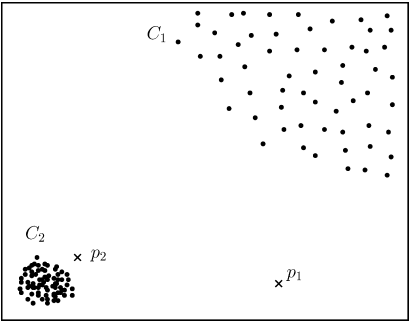
\includegraphics{chap01/localvsglobal.png}
		\caption{Limitations of Global outlier detection}
	\end{figure}
	
	
	
	\par 
	Local density based outlier detection is preferred over global because global density based techniques performs poorly for datasets with varying densities.
	Consider the 2-D data set shown in Figure 2.1, both points p1 and p2 should be detected as outliers. But if we consider global density, p2 will not be detected as outlier because of low density of cluster C1. For a point q in cluster C1, the distance between q and its nearest neighbor will always be greater than distance between p2 and its nearest neighbor.
	


	
	
	\section{Incremental Local Outlier Detection for Data Streams}
	Incremental LOF for data streams refer to computation LOF score of newly added data points and updating the same for older data points. Outlier detection techniques are categorized into 4 types \cite{f}
	
	\begin{enumerate}
		\item \textit{Statistical Approach} : the data points are typically modeled using a stochastic distribution, and points are labeled as outliers depending on their relationship with this model.
		
		\item \textit{Distance Based Approach} : detect outliers by computing distances among points.
		
		\item \textit{Profiling Methods} : Profiles of normal behavior is built and deviation from that are considered outliers.
		
		\item \textit{Model-based Approach} : First characterization of normal points using predictive models like neural networks and SVM. Deviation from these models are considered outliers.
		
		
	\end{enumerate}
	
	Static LOF algorithms can be applied to data stream is three ways. However these are computationally inefficient.
	
	\begin{enumerate}
		\item \textit{Periodic LOF} : Static LOF is applied periodically on entire data set every time new data blocks are entered. The problem with such approach is that a data point which may be anomalous while added may not be detected as outlier later as many other points are added. they may create a cluster of their own and outliers will be missed. If LOF is computed each time a data point is added, the change is behavior can be detected at that moment.
		
		\item \textit{Supervised LOF} : K-distance, lrd and LOF of the data points are precomputed. Any new data point that arrives all these parameters are computed without updating for previous points. As a result the LOF accuracy decreases. 
		
		\item \textit{Iterated LOF} : Aplpy static LOF every time a new data point enters. This gives high accuracy at a cost of very high computational time. 
		
		
	\end{enumerate} 
	

	\begin{algorithm}[H]
		\caption{iLOF Insertion}
		\begin{algorithmic}
			\STATE  
			\STATE INPUT:  A data point $p_t$ at time t
			\STATE OUTPUT: LOF value LOF($p_t$)
			\STATE
			
			\STATE Compute KNN and K-distance of $p_t$
			
			\FOR {all o \in KNN($p_t$)}	
			
			\STATE Compute \texttt{reach-dist($p_t$,o)}
			
			\ENDFOR
			
			\STATE  $S_{update}$ \leftarrow Reverse KNNs of $p_t$
			
			\FOR{ all o \in $S_{update}$ and q \in $N_{(o,k)}$}
			
			\STATE Update K-distance(o) and reach-dist(q,o)
			
			\IF {o \in  $N_{(q,k)}$}
			
			\STATE $S_{update}$ \leftarrow  $S_{update}$ \cup q
			\ENDIF
			
			\ENDFOR
			
			\FOR { all o \in $S_{update}$ }
			
			\STATE Update lrd(o) and LOF(R-KNN(o,k))
			
			\ENDFOR
			\STATE Compute lrd($p_t$) and LOF($p_t$)
			\RETURN LOF
			
			
		\end{algorithmic}
	\end{algorithm}

In Incremental approach, LOF score is computed as soon as a data enters. It is determined whether it is outlier or not. LOF of other data points are also updated. 


The algorithm for insertion of a data point in iLOF is given in Algorithm 1. First we compute the K nearest neighbors of new point $p_t$. To update the led and LOf of affected points we compute the reverse K nearest neighbors(RKNN) of these points. All these points are kept in an array called $S_update$. Finally for all these points, lrd and LOF value is computed.  

	

\section{Dolphin}

Dolphin is a distance based outlier detection technique for disk resident datasets. The algorithm receives
as input a disk-resident dataset DS and parameters k and R, and outputs all
and only the DB(k,R) outliers of DS. Dolphin does two scans to find all the outlier points \cite{e}.

\subsection{Algorithm}

DOLPHIN gains efficiency by naturally merging together in a unified
schema three strategies, namely

\begin{enumerate}
	\item 
	The selection policy of objects to be maintained in main memory
	
	\item Usage of pruning rules
	\item Similarity search techniques
\end{enumerate}


Dolphin uses a part of the main memory and loads a part of the dataset. It maintains a data structure called INDEX while scanning. According to Dolphin , points which do not have at least K points in the radius of R are considered anomalous. Each DBO(Distance Based Outliers) node in INDEX data structure contains

\begin{enumerate}
	\item n.obj : Original Object 
	\item n.id : id of object 
	\item n.nn[h] : an integer array  
\end{enumerate}

n.nn[i] is the number of points which lie at a distance of  \[ \bigg[   {\frac{R}{h}} (i-1) , {\frac{R}{h} } i \bigg] \]  from n.obj.

\[  n.rad = {\frac{R}{h}} i  \ \ \ \           (1 \leq i \leq h) \]
where i i sthe smallest integer such that 

\[  \sum_{j \leq i} n.nn[j]  \ \ \      is \ at \ least \ K-1 \]



After the scan INDEX contains all the outliers but all the points in INDEX need not be outliers. In second scan inliers are removed from INDEX by calling pruneInliers.

\begin{algorithm}[H]
	\caption{Algorithm}
	\begin{algorithmic}
		\STATE  
		\STATE INPUT:  DS Disk Resident Datasets
		\STATE OUTPUT: INDEX containing all the outliers
		\STATE
		
		\STATE Initialize empty INDEX
		
		\FOR {all obj \in DS($p_t$)}	
		
			\STATE $n_{curr}$  $\leftarrow$ obj
			\IF{ ! isInlier( $n_{curr}$ ) }
				\STATE Insert $n_{curr}$ in INDEX
			\ENDIF
		
		\ENDFOR
	
	\STATE  remove from INDEX all the nodes such that n.rad  R
	\STATE  Reset n.nn for all
		
	\end{algorithmic}
\end{algorithm}

In first scan each of the incoming data point, it is decided whether a it is inlier or not by computing distances from the points already in INDEX. If it is not inlier then it is inserted in INDEX. So after first iteration INDEX contains all the outliers. But all the points in INDEX may or may not be outliers. We prune these normal points from INDEX in second scan. In second scan proved inlier are removed and candidate outliers are examined again.  Finally only outliers are present in INDEX.

\begin{algorithm}[H]
	\caption{IsInlier}
	\begin{algorithmic}
		\STATE  
		\STATE INPUT:  $n_{curr}$
		\STATE OUTPUT: Binary (True/Flase)
		\STATE
		
		\STATE Range query search in INDEX
		
		\FOR {all $n_{index}$ \in INDEX}	
		
			\STATE   dst= d($n_{index}$.obj,$n_{curr}$.obj)
			\IF{dst<R-$n_{index}$.rad}
				\RETURN True
			\ENDIF
			
			
			\IF{dst<R}
				\STATE oldRad=$n_{index}$.rad
				\STATE update $n_{index}$.nn[]
				
				\IF{oldRad $>$ R AND $n_{index}$.rad $<$ R}
				 	\STATE  Remove $n_{index}$ from INDEX
				\ENDIF
				
			
			\ENDIF
			
			\STATE  Update $n_{curr}$.nn[]
			
			\IF{$n_{index}$.rad $<$ R}
			   \STATE {$n_{index}$.rad $<$ R} 
			\ENDIF
			
		
		\ENDFOR
		
		\RETURN False
	\end{algorithmic}
\end{algorithm}



\begin{algorithm}[H]
	\caption{PruneInliners}
	\begin{algorithmic}
		\STATE  
		\STATE INPUT: obj
		\STATE
		
		\STATE Range query search in INDEX whith center obj and Radius R
		
		\FOR{ $n_{index}$}
		    \IF {d(bj,$n_{index}$.obj) $<$ R}
	            \STATE Update $n_{index}$.nn[]
 		    \ENDIF
 		    
 		    \IF{$n_{index}$.rad $<$ R}
 		    	\STATE remove $n_{index}$ from INDEX
 		    \ENDIF
		\ENDFOR
		
	\end{algorithmic}
\end{algorithm}


\subsection{Pivoting Based Search Algorithm}

Instead of computing all pairwise distances between points, some pivot points are taken and pairwise distance between all other points are computed. If we have to find distance between two points x and y ,according to triangles inequality

\[  d(x,y) \geq |{d(x,p) - d(y,p)}| \]

\[  d(x,y) \geq D_p(x,y) \]


\[ D(x,y) =MAX_{1 < i <m} D_p(x,y) \]

$D_p(x,y)$ is lower bound of d(x,y). We need to find y such that D(x,y) $<$ R. This returns a superset of y such that d(x,y) $<$ R.





\section{Memory Efficient Incremental Local Outlier Factor (MiLOF)}

Local Outliers detection in data streams when limited memory is available. It is impractical to store all the instances of data streams. Some of the points has to be removed and summarized. Memory available is just sufficient to store K-Distance, lrd and LOF of m data points only.

The available m memory is divided in two parts of size b and c to store original points and summarized points respectively. When memory limit is reached, first ${\frac{b}{2}}$  data points are summarized to c clusters and deleted to free memory \cite{d}. If there already exists summarized data, the old and new cluster centers are merged. Hence at any time maximum memory used is b=m+c.
 Three steps of MiLOF are 

\subsection{Summarization}
Whenever memory reaches limit b, summarization phase is invoked. This phase summarizes first ${\frac{b}{2}}$ points, their K-distance, lrd and LOF and deletes these points from memory. Recent points are retained because data points might have evolved with time and recent points are most important. As the width of the summarization window decreases, it resembles iLOF. So MiLOF is direct generalization of iLOF.

\par 
Summarization  is explained in algorithm 5.
In summarization, if memory is reached first $\frac{b}{2}$ points are summarized to c clusters. K-distance, lrd and LOF for these cluster centers are computed by the following formulas.  

\begin{itemize}
	\item K-Distance of cluster center $v^i_j$ \in $V^i$ 
	
	
		\[  K-Distance(v^i_j) = \frac{\sum_{p \in C^i_j } K-Distance(p)}{| C^i |} \]
		
		
	 \item lrd of cluster center $v^i_j$ \in $V^i$ 
		
		
		\[  lrd_k(v^i_j) = \frac{\sum_{p \in C^i_j } lrd_k(p)}{| C^i |} \]
		
		\item LOF of cluster center $v^i_j$ \in $V^i$ 
		
		
		\[  LOF_k(v^i_j) = \frac{\sum_{p \in C^i_j } LOF_k(p)}{| C^i |} \]
	
\end{itemize}


\begin{algorithm}[h!]
	\caption{MiLOF}
	\begin{algorithmic}
		\STATE  
		\STATE INPUT:  A data point p 
		\STATE OUTPUT: LOF value LOF(p)
		\STATE
		
		\STATE Compute LOF of p 
		\IF {No of points=b}
			\STATE $C^i$ $\leftarrow$ First $\frac{b}{2}$ points
			\STATE ($V^i$,$N^i$) $\leftarrow$ C-means($C^i$)
			
			\FOR {all $v^i$ \in $V^i$} 
			  \STATE Compute avereage K-distance, lrd and LOF
			\ENDFOR
			
			\STATE Delete $C^i$
			
			\IF{i>0}
				\STATE (Z;W) $\leftarrow$ Weighted c-means($V^i$ U $V^{i-1}$ ,$N^i$ U $N^{i-1}$)
				
				\FOR {all z \in Z} 
					\STATE Compute avereage K-distance, lrd and LOF
				\ENDFOR 
				\STATE $V^{i-1}$ \leftarrow Z
				\STATE Delete $V^{i-1}$,Z
				
			\ENDIF	
		\ENDIF
		
		\STATE i $\leftarrow$ i+1
		\RETURN LOF
	\end{algorithmic}
\end{algorithm}

\subsection{Merging}

Summarization is performed every time new $\frac{b}{2}$ new data points arrives. Clustering these points gives c cluster centers $V^i$. These clusters are to be merged with old c cluster centers $V{i-1}$ so that finally only c centers are available. Cluster centers X={$V^i$ U $V^{i-1}$} are merged using a weighted clustering algorithm where weight of each center is no of objects in that cluster. 


\subsection{Revised Insertion}
Whenever a new data points arrives, LOF value for it is computed similar to iLOF with only difference that iLOF uses only data points to compute LOF where as in revised insertion we use both the data points and the cluster centers. While calculating the KNN, if any of the point is cluster center then it is assumed that all other nearest neighbor belongs to the same cluster. Hence distance from the point and that cluster center is taken as the K-distance for that point.  

